\section{Introduction}
The primary area of study that this research project takes place in is differential geometry and topology. One of the most important concepts, not just in differential geometry and topology, but in almost all areas of mathematics, is that of a \textit{manifold}. At this point, it will suffice if the reader considers the surface of a sphere or torus.\\

\begin{figure}[h!]
\centering
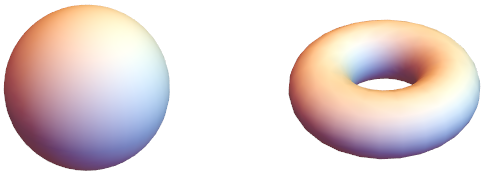
\includegraphics[scale=0.675]{fig/fig1a}
\caption{The sphere and torus are examples of manifolds.}
\end{figure}

If one were to cut out a small piece of one of these surfaces, then it would look like a flat sheet of paper. Since this sheet of paper is two-dimensional, we think of these surfaces as being two-dimensional as well. What makes the study of manifolds interesting however, is in what is happening at a \textit{global} scale: \textit{locally} a piece of the sphere looks like the flat Euclidean plane but \textit{globally} the sphere is clearly not flat and standard notions from Euclidean geometry no longer apply. For example, if one takes two parallel lines on the surface of a sphere (where a ``line'' is no longer necessarily a straight line but still has the meaning of shortest path between two points) and continue along them for long enough, they will eventually meet. For instance, imagine two lines that point due north from the equator - they will start out parallel but will intersect at the north pole.\\

\begin{figure}[h!]
\centering
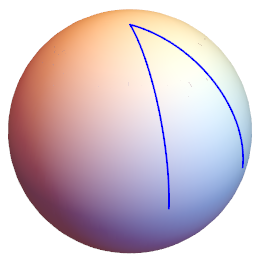
\includegraphics[scale=0.675]{fig/fig2a}
\caption{Two lines starting out parallel on the sphere will eventually intersect.}
\end{figure}

These examples of the sphere and torus are usually visualised quite naturally as surfaces ``sitting'' in three-dimensional space but often we will talk about manifolds as intrinsic objects - not necessarily embedded in any higher space. Furthermore, there is nothing stopping us from talking about manifolds of any arbitrary dimension, and while a seven dimensional sphere may be hard to visualise, such higher-dimensional objects are of central importance to this project.\\

\pagebreak

One important task when working with abstract manifolds is the choice of a local coordinate system so that explicit computations may be carried out on the manifold. As a motivating example, consider $\mathbb{S}^2$. We can think of each point on $\mathbb{S}^2$ as the origin of its tangent space. One must decide how to draw an $x$-axis and a $y$-axis, as well as the positive and negative directions along each axis. This information can be encoded by two arrows, one pointing along the $x$-axis in the positive direction and one pointing along the $y$-axis in the positive direction. A natural question to ask arises, namely:
\begin{center}
\textit{Can we choose our arrows at each point of our space in such a way that they vary smoothly when the points themselves vary smoothly?}
\end{center} 
If we can make such a choice, our space is said to be \textit{parallelisable}.

In Section 3.1, in the case of $\mathbb{S}^2$, it is show that such a choice cannot be made. It is then shown that this is in fact true of all even dimensional spheres. Furthermore, we will find that the only spheres that do admit such a choice are $\mathbb{S}^1$, $\mathbb{S}^3$ and $\mathbb{S}^7$. Strictly speaking $\mathbb{S}^0$ also admits such a choice, however is considered a trivial case.

%Fundamentally, we are interested in answering the question:
%\begin{center}
%\textit{Which spheres admit a parallelisation?}
%\end{center}
\subsection{Literature Review and Historical Overview}
As previously stated, a classic result of algebraic topology due to Brouwer in 1912 \cite{MR1511678} is that in the case of the two-dimensional sphere $\mathbb{S}^2$, we cannot make such a choice. This result came to be known as the ``Hairy Ball Theorem'', since it can be thought of as saying that there is no way to comb the hair of a coconut (or someone's head) without creating a cowlick. It is also worth noting that Brouwer's original proof made use of cohomology theory and other tools from algebraic topology \cite{MR1415833}. Milnor gave a new, more analytic, proof of the theorem in 1978 \cite{MR505523}.\\

One of the results that we will show in the latter sections of this report is that this result generalises, in that it is not possible to make such a choice of arrows on any sphere of even dimension (equivalently, only spheres of odd dimension admit the existence of, at least one, everywhere non-zero smooth vector field). 
%The proof presented is due mainly to \cite{burger2016riemannian} and is nice in its use of relatively elementary differential geometry and analytic methods.\\
What we find in the case of $\mathbb{S}^3$ the three-dimensional sphere however, is quite different. We can think of $\mathbb{S}^3$ as the collection of all points of the form $(x,y,z,w)$ unit distance from the origin, such that $x^2+y^2+z^2+w^2=1$. Each point of the 3-sphere can now be regarded as an object known as a \textit{quaternion}, which are a type of number developed in 1843 by William Hamilton \cite{hamilton1844ii}.\\

Quaternions are similar in nature to complex numbers, but we now introduce three distinct numbers, denoted usually by $i,j,k$, each with the property $i=j=k=\sqrt{-1}$. Unlike real or complex numbers however, the order in which one multiplies quaternions matters; this is to say that $ij=k$ but $ji=-k$. The quaternion associated with the point $(x,y,z,w)$ is $x+yi+zj+wk$ and if $x^2+y^2+z^2+w^2=1$, then it is called a \textit{union quaternion}.
It can be shown that multiplying two unit quaternions together results in another unit quaternion. Furthermore, given any unit quaternion $q$, the three (unit) quaternions given by $iq$, $jq$ and $kq$ are all perpendicular to $q$. Therefore, one can use these quaternions as directions for the three axes needed for the tangent space at $q$ and that they do vary smoothly as the point $q$ varies.\\

One may then be curious as to whether this type of construction generalises to higher dimension. That is, through some notion of `nice multiplication' of points on the sphere. Assuming we wish to use a conventional number system, we have at our disposal the real numbers, the complex numbers (which give us a result for the parallelisability of $\mathbb{S}^1$), the quaternions and then the \textit{octonions} (sometimes referred to as \textit{Cayley numbers}). The octonions are an eight-dimensional number system again similar in nature to the complex numbers and quaternions. Since the octonions are eight-dimensional, the unit octonions form a seven-dimensional sphere, which will be shown to be parallelisable through a similar method to that for $\mathbb{S}^1$ and $\mathbb{S}^3$.\\
 
%\begin{center}
%\textbf{HURWITZ, CAYLEY, OCTONIONS}
%\end{center} 
A theorem of Hurwitz, proved in 1898 \cite{Hurwitz1898,Hurwitz1923}, implies that multiplicative formulae for sums of squares can only occur in dimensions 1, 2, 4 and 8. It is now known that these dimensions are those in which systems known as \textit{normed division algebras} exist. It was not however, until 1940/1941 when Hopf showed that the dimension of a division algebra must be a power of 2, \cite{MR0004785}. Then later, in 1958, Milnor managed to show that it is in fact only in dimensions 1, 2, 4 and 8 do these division algebras exist \cite{MR0102805}.\\

The fact that there are not any more number systems of this type for other dimensions does not immediately show that spheres in those other dimensions are not parallelisable, since there might be some other method for choosing our vectors. However, once again Milnor and Bott \cite{MR0102804} were able to show in 1958 that 1, 2, 4 and 8 are in fact the only dimensions in which a sphere is parallelisable. Hirzebruch and Kervaire also arrived at the same result independently \cite{MR1415833,MR3075371,atiyah1961bott}.\\

%This is the other main result which we show in the main report. 
The proof that $\mathbb{S}^n$ for $n=1,3,7$ are parallelisable is given in Section 3.3 and utilises the aforementioned existence of a well defined multiplication that is closed on these spheres. Unfortunately, it is beyond the scope of this research project to show that these are indeed the \textit{only} parallelisable spheres, due to the highly technical machinery involved. The proof that these are the only parallelisable spheres is due to Adams \cite{MR0141119}. We briefly discuss this in Section 4.\\

Sphere parallelisability is closely related to the work of Hopf and specifically the notion of \textit{Hopf fibrations} which are examples of fibre bundles. Fibre bundles are a generalisation of a concept discussed in Section 2.3. For the moment, it will suffice to describe them as spaces that are characterised by being \text{locally} a product space, but may have a different \textit{global} topological structure. \\

%\pagebreak

As discussed in the following sections, the technical definition of a parallelisable manifold is one for which the tangent bundle (a type of fibre bundle associated with the tangent space of a manifold) is `trivial'.\\

The Hopf fibrations are examples of fibre bundles where the base, total and fibre spaces are all spheres. Through the results of Adams \cite{MR0141119}, we find that there are precisely four Hopf fibrations, and in particular, each Hopf fibration's fibre space are exactly the parallelisable spheres: $\mathbb{S}^0$, $\mathbb{S}^1$, $\mathbb{S}^3$ and $\mathbb{S}^7$.\\

\pagebreak

Hopf's 1931 paper, \cite{MR1512691} introduced a map from the 3-sphere to the 2-sphere which describes the 3-sphere in terms of a union of disjoint, interlocking circles (the fibres of the fibre bundle), each circle corresponding to a point on the 2-sphere. In Hopf's follow up paper \cite{Hopf1935}, he generalised this result. However, as previously stated, it wasn't until the work of Adams in 1960 and his papers \cite{MR0141119,MR0139178} from which it followed that these were the only four such fibrations.\\

%\section{Reviews of Secondary Literature}
%Regarding Milnor's analytic proof of the hairy ball theorem for $\mathbb{S}^2$:

%\textit{Milnor gives elementary analytic proofs of the theorems mentioned in the
%title. The key idea used is a computation to show that, for small values of a variable $t$ and for $x\to v(x)$ a smooth vector field defined on a neighborhood of a subset $A\subset \mathbb{R}^n$, the mapping $f_t(x) = x+tv(x)$ is one-to-one and maps $A$ onto a region whose volume can be expressed as a polynomial function of $t$.}
%
%Relevance?\\
An article that discusses some of the history behind Hopf's discovery is given in \cite{MR1721115}\footnote{The curious reader is encouraged to peruse this paper, since it really is quite an interesting read.}
The paper describes how the early work of Clifford and Klein influenced Hopf's discovery of a mapping from the 3-sphere to the 2-sphere. In 1873, Klein saw Clifford deliver a lecture on a surface of ``zero curvature and infinite extent''. Klein went on to publish some of these ideas in an 1890 paper on non-Euclidean geometry. Hopf learned of these ideas through his involvement in the (posthumous) publication of Klein's book \textit{Non-Euclidean geometry}. The paper also includes a letter from Hopf to Hopf’s first doctoral student Freudenthal describing the homotopy classes of maps from $\mathbb{S}^3$ to $\mathbb{S}^2$.\footnote{Adapted from a review, available via MathSciNet, reference I.D: MR1721115.}
\pagebreak
